\chapter{Full CLs Shape-Based Limits
\label{ch:limits}}

To set limits using the modified frequentist $\text{CL}_{s}$ procedure \cite{Read:CLs}, two hypotheses are defined. The first is the null or background-only hypothesis $H_{0}$ or $b$, and the second is the alternate or signal plus background hypothesis $H_{1}$ or $s+b$.

$\mathcal{P}(\theta; N_{H_{i}})$ is defined as the Poisson probability to observe $\theta$ events in data given the hypothesis $H_{i}$ which predicts $N_{H_{i}}$ events. This probability can be defined generally for the whole sample, but also per bin for a histogram of some quantity, e.g. \ST, and/or per channel.

To obtain this probability, it is necessary to integrate over all of the nuisance parameters:
\begin{equation}
\mathcal{P}(\theta; N_{H_{i}}) = \int \mbox{Poisson}(\theta; N_{H_{i}},\eta)f(\eta)d\eta
\end{equation}
where $f$ is the probability density function (PDF) for the nuisance parameter $\eta$.

With those definitions, the test statistic $\mathcal{Q}$ is written as a ratio of likelihoods for a basic counting experiment:
\begin{equation}
\mathcal{Q} = \frac{\mathcal{P}(\theta; N_{H_{1}})}{\mathcal{P}(\theta; N_{H_{0}})}
\end{equation}
Splitting into bins and channel gives:
\begin{equation}
\mathcal{Q} = \prod_{i=e,\mu}\prod_{j=0}^{n_{\text{bin}}} \frac{\mathcal{P}_{i,j}(\theta; N_{H_{1}})}{\mathcal{P}_{i,j}(\theta; N_{H_{0}})}
\end{equation}
For simplicity of computation, another form of the test statistic can be defined using the log likelihood ratio:
\begin{equation}
q = -2 \ln \mathcal{Q}
\end{equation}

To evaluate the test statistic as a function of the number of observed events $\theta$, many simulated pseudo-experiments are performed. For each hypothesis, $\theta$ is varied according to the probability distribution of that hypothesis, and the value of $\mathcal{Q}$ (or $q$) is kept for each $\theta$ value. To get $\mathcal{Q}$ for the actual number of observed events, $\mathcal{Q}_{\text{obs}}$, the same procedure is followed using $\theta=N_{\text{obs}}$. The $\text{CL}_{s+b}$ and $\text{CL}_{b}$ variables correspond to the probability for $\mathcal{Q_{\text{obs}}}$ to be greater than the $\mathcal{Q}$ values obtained for the hypotheses $H_1$ and $H_0$, respectively. When using $q$, the observed value should be smaller than the value for the hypothesis. A visual example of these variables is shown in Fig. \ref{fig:q}.
\begin{align}
\text{CL}_{s+b} &= \mathcal{P}(\mathcal{Q} \leq \mathcal{Q}_{obs}|H_1) = \mathcal{P}(q \geq q_{obs}|H_1) \\
\text{CL}_{b} &= \mathcal{P}(\mathcal{Q} \leq \mathcal{Q}_{obs}|H_0) = \mathcal{P}(q \geq q_{obs}|H_0) \\
\text{CL}_{s} &= \text{CL}_{s+b}/\text{CL}_{b}
\end{align}

\begin{figure}[hbt]
\begin{center}
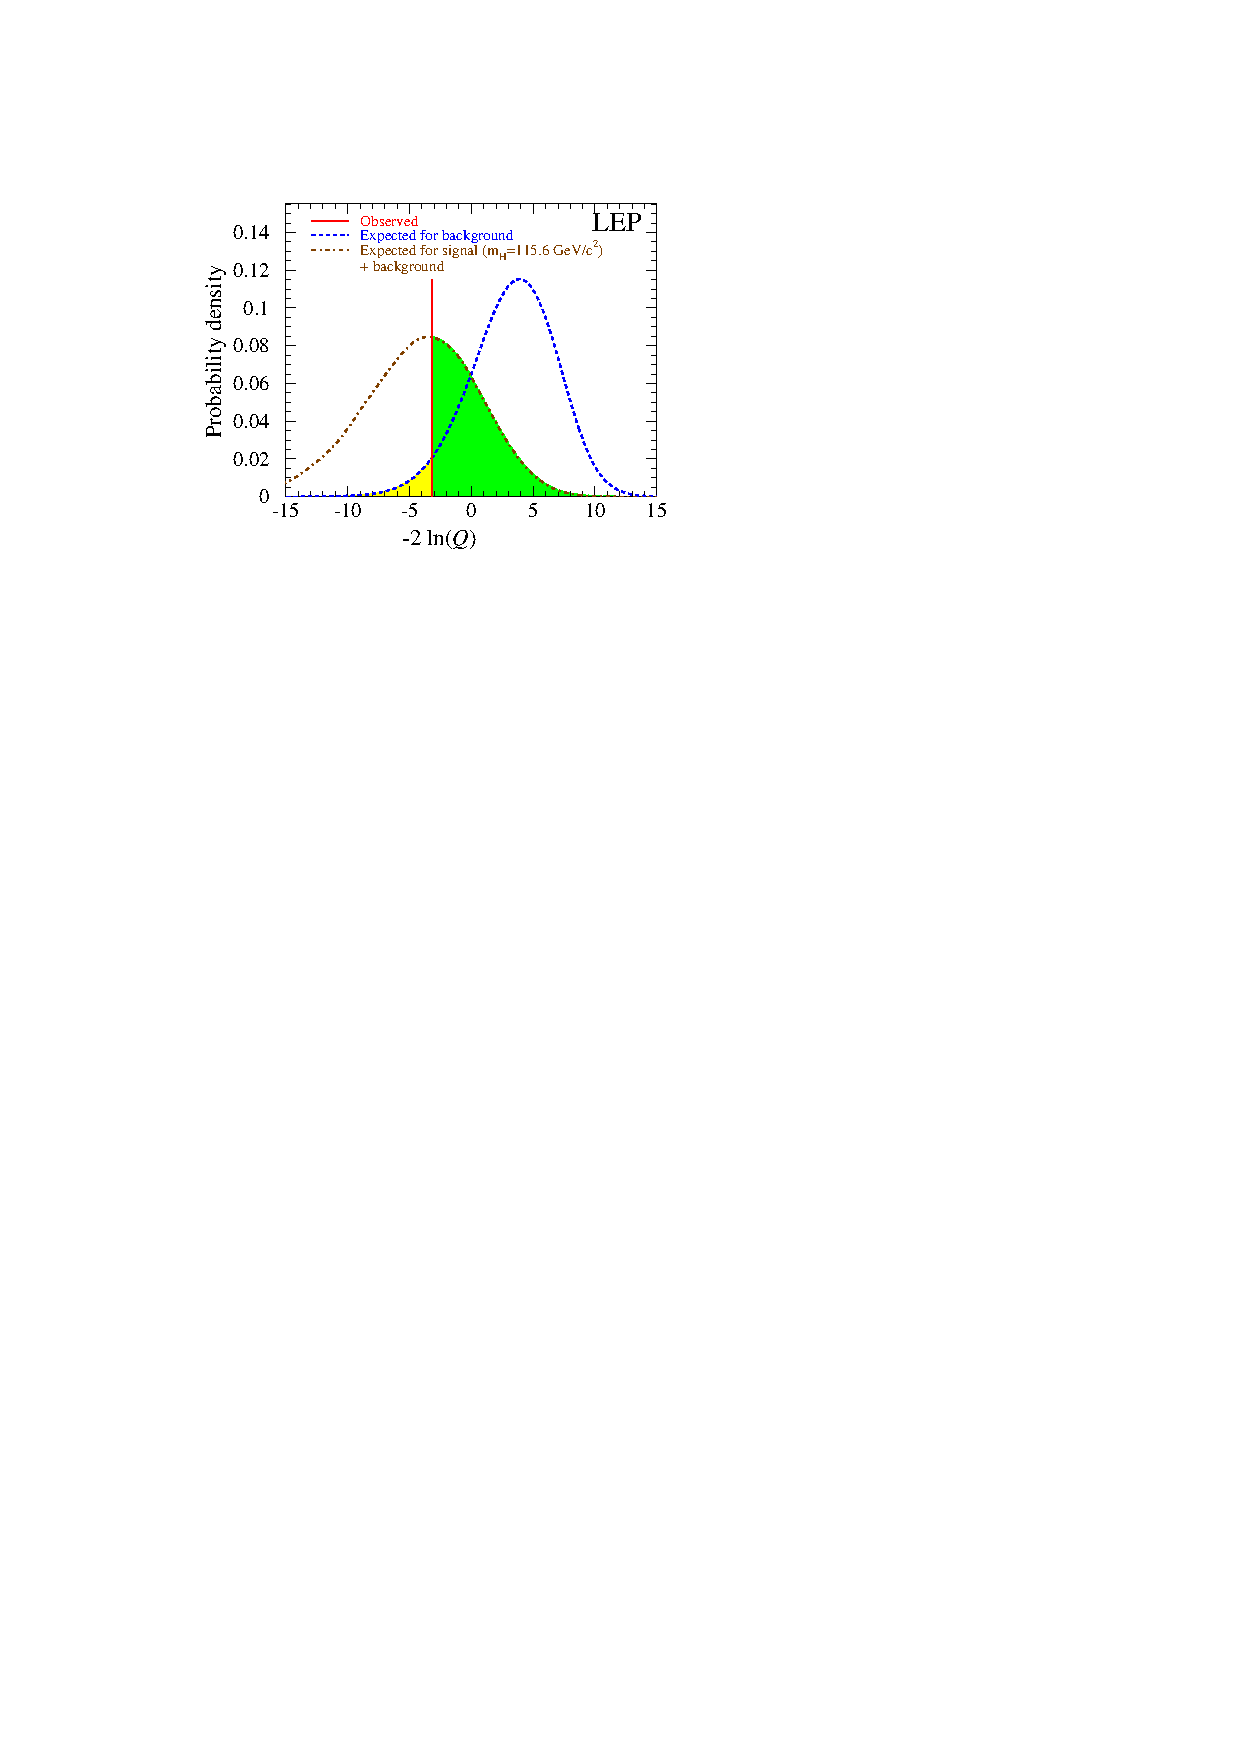
\includegraphics[width=0.95\textwidth]{figures/g21013-fig1.pdf}
\caption{Comparison of the observed value (red line) to the probability densities for $H_{0}$ (background only, blue line) and $H_{1}$ (signal + background, brown line) as a function of the log likelihood ratio. Green area: $\text{CL}_{s+b}$, yellow area: $1-\text{CL}_{b}$. From \cite{Read:presentation}.}
\label{fig:q}
\end{center}
\end{figure}

To set a mass limit on the signal hypothesis, the calculation of $\text{CL}_{s}$ is repeated for different signal masses. Masses with $\text{CL}_{s} < 1 - \alpha$ are excluded at the $\alpha$ confidence level, typically 95\%.